\section{Proprietà degli stimatori}
Gli stimatori possono godere di alcune proprietà. Le proprietà di maggiore interesse sono:
  \begin{itemize}
     \item polarizzazione
     \item consistenza
     \item asintottica normalità
   \end{itemize}
% ######################################################################## Polarizzazione
\subsection{Polarizzazione}
La polarizzazione \index{Polarizzazione} indica lo scostamento della stima $\hat{\theta}$ rispetto al valore esatto $\theta^0$: se uno stimatore è non polarizzato, non c'è alcun scostamento rispetto al valore esatto e la sua ddp è centrata su di esso quindi $E[\hat{\theta}]=\theta^0$; altrimenti è polarizzato e scriviamo $E[\hat{\theta}]\ne \theta^0$. In figura \ref{fig:espolarizzazione} lo stimatore $f_{\hat{\theta}_1}$ è non polarizzato, mentre lo stimatore $f_{\hat{\theta}_2}$ è polarizzato. 

  \begin{figure}[htbp]
    \centering
    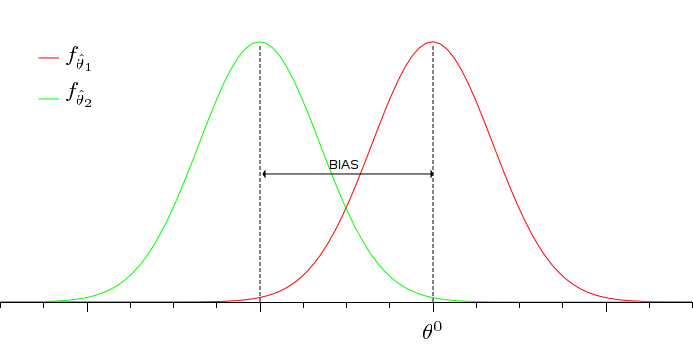
\includegraphics[scale=1]{mathematica/polarizzazione}
    \caption{esempio di polarizzazione\label{fig:espolarizzazione}}
  \end{figure}

In uno stimatore polarizzato, la differenza fra il valore atteso dello stimatore ed il valore vero è definito BIAS:

    \[ BIAS=E[\hat{\theta}]-\theta^0 \]

In linea di massima è preferibile uno stimatore non polarizzato, ma esistono alcuni casi in cui può essere conveniente usare uno stimatore polarizzato. 


% ######################################################################## Consistenza
\subsection{Consistenza}
La consistenza \index{Consistenza} è una proprietà molto desiderabile in quanto essa definisce la capacità di uno stimatore di concentrare i propri valori al crescere del numero di campioni considerati in un esperimento; se uno stimatore è consistente, per grandi campioni, avremo una varianza piccola attorno ad un valore e quindi una migliore stima, inoltre, se lo stimatore è non polarizzato all'aumentare dei campioni questi tendono a concentrarsi attorno al valore esatto \footnote{Idealmente per infiniti campioni diventa una delta di Dirac su valore esatto} come rappresentato in figura \ref{fig:esconsistenza}

\begin{figure}[htbp]
  \centering
  \includegraphics[scale=1]{mathematica/consistenza}
  \caption{esempio consistenza\label{fig:esconsistenza}}
\end{figure}

% ########################################################################
\subsection{Asintottica normalità}
L'asintotica normalità \index{Asintottica normalità}, definisce la capacità di uno stimatore di tendere ad una distribuzione gaussiana all'aumentare dei campioni acquisiti.
% ######################################################################## disuguaglianza CR
\subsection{Disuguaglianza di Cramer-Rao}
Con la disuguaglianza di Cramer-Rao \index{Limite Cramer Rao} - CR - si definisce un limite inferiore per la varianza oltre il quale la stima non può migliorare:

    \[ Var[\hat{\theta}]\geq - \left( E\left[\frac{\partial^2}{\partial\theta^2} ln f_X^\theta(X)\mid_{\theta=\theta^0}\right] \right)^{-1} = S^{-1} \]

Per uno stimatore non polarizzato la varianza è sinonimo di precisione, quinidi, una varianza minore significa maggiore precisione e quindi è da preferire. Da questa disuguaglianza ne consegue che non è possibile ottenere uno stimatore con una varianza inferiore al limite di CR. Il limite CR esiste perché, dopotutto, dai dati sperimentali non si può ricavare più di tanto e un marg    ine di incertezza rimane sempre: il risultato ideale a varianza nulla è impossibile da ricavare puntualmente.\newline
La quantità utilizzata per definire il limite CR è detta \textit{quantità di informazione di Fisher} \index{Quantità di informazione di Fisher}:

    \[ S:= -  E\left[\frac{\partial^2}{\partial \theta^2} ln f_X^\theta(X)\mid_{\theta=\theta^0}\right] \]

Per un caso vettoriale, avremo una matrice di informazione:

\begin{gather*}
  S= \{ S_{ij}\}  \\
  S_{ij}:= -  E\left[\frac{\partial^2}{\partial \theta_i\partial \theta_j} ln f_X^\theta(X)\mid_{\theta=\theta^0}\right]
\end{gather*}

Il limite CR è definito solo per stimatori non polarizzati, ma esiste una legge analoga anche per il caso di stimatori polarizzati.
% ######################################################################## Conclusioni
\subsection{Conclusioni}
Come prima osservazione, uno stimatore inconsistente deve destare sospetti perché non riusciremmo a stimare precisamente un parametro dato che all'aumentare dei campioni non ci vengono fornite nuove informazioni, mentre è desiderabile che avvenga il contrario fino a tendere ad una stima precisa.\newline
Generalmente, come già accennato, è preferibile uno stimatore non polarizzato, ma potrebbe capitare che sia più utile uno polarizzato; ad esempio potrebbe essere preferibile uno stimatore poco polarizzato ma che ha una varianza molto piccola rispetto ad uno stimatore non polarizzato ma con un'ampia varianza.

\begin{figure}[htbp]
  \centering
  \includegraphics[scale=1]{mathematica/polarizzazione2}
  \caption{Confronto fra stimatore polarizzato consistente e uno non polarizzato e non consistente\label{fig:confrontopolarizzazioneconsistenza}}
\end{figure}

Come si vede in figura \ref{fig:confrontopolarizzazioneconsistenza}, nel caso dello stimatore polarizzato $f_{\hat{\theta}_2}$, i valori che ci vengo forniti sono in un intorno piccolo vicino al valore esatto, quindi anche se sappiamo di sbagliare la stima, sappiamo anche che stiamo sbagliando di poco rispetto allo stimatore non polarizzato $f_{\hat{\theta}_1}$ che invece ha un ampio margine di errore. Infatti, lo stimatore polarizzato è più consistente rispetto al non polarizzato e come visto in precedenza, la consistenza è una proprietà molto desiderabile. L'ideale sarebbe spostare lo stimatore polarizzato di modo da centrarlo e quindi renderlo non polarizzato.\newline
Abbiamo appena dimostrato che uno stimatore polarizzato potrebbe essere preferibile, ma come possiamo valutare analiticamente la sua precisione? Quello che possiamo fare è valutare l'errore quadratico medio (mean square error):

    \[ E[(\hat{\theta}-\theta^0)^2] \approxeq 0\]

Il motivo per cui si valuta l'errore quadratico e non l'errore, è che valutando l'errore è facile ottenere $E[\hat{\theta}-\theta^0]=0$ mediante compensazione fra errori positivi ed errori negativi, mentre con l'errore quadratico ciò non capita.

    \[
        \begin{split}
            E[(\hat{\theta}-\theta^0)^2]&=E[(\hat{\theta}-E[\hat{\theta}])+(E[\hat{\theta}]-\theta^0)^2]=\\
            &=Var[\hat{\theta}]+2E[(\hat{\theta}-E[\hat{\theta}])](E[\hat{\theta}]-\theta^0)+(E[\hat{\theta}]-\theta^0)^2=\\
            &=Var[\hat{\theta}]+(E[\hat{\theta}]-\theta^0)^2
        \end{split}
    \]
    
Dalla formula appena illustrata, possiamo concludere che lo stimatore polarizzato è accettabile se si guadagna abbastanza in varianza o, viceversa, preferire la non polarizzazione perdendo in varianza. Uno stimatore non polarizzato $\hat{\theta}^m$ si dice a minima varianza \index{minima varianza} se:

    \[ Var[\hat{\theta}^m]\leq Var[\hat{\theta}],\quad\forall \hat{\theta} \]

Questo significa che lo stimatore non polarizzato è a minima varianza se la sua varianza è minore, o uguale, alla varianza di un qualisasi altro stimatore non polarizzato. Se uno stimatore ha la varianza che raggiunge il limite CR \index{Limite Cramer Rao} allora è sicuramente a varianza minima; non è detto che ogni stimatore possa raggiungere il limite CR, ma ciò non vieta l'esistenza della minima varianza.
